\documentclass[11pt,a4paper]{article}

% Packages
\usepackage[utf8]{inputenc}
\usepackage[english]{babel}
\usepackage{graphicx}
\usepackage{geometry}
\usepackage{float}
\usepackage{subcaption}

% High-quality image rendering
\pdfimageresolution=600

% Page setup
\geometry{margin=0.75in}
\setlength{\parindent}{0pt}
\setlength{\parskip}{10pt}

% Title information
\title{\textbf{Lab 3 - Data Preparation Report}}
\author{}
\date{}

\begin{document}

\maketitle

% ============================================================
\section{Traffic Accidents Dataset}
% ============================================================

% ------------------------------------------------------------
\subsection{Step 1: Variable Encoding}
% ------------------------------------------------------------

\begin{figure}[H]
\centering
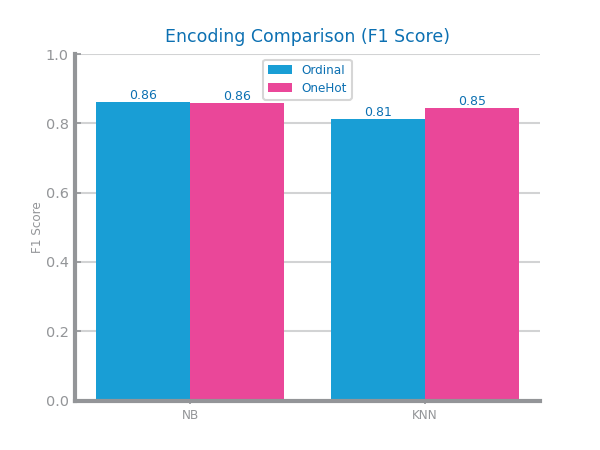
\includegraphics[width=0.85\textwidth]{../images/lab3/traffic_accidents/1_encoding_comparison.png}
\caption{Encoding approaches comparison - Traffic Accidents}
\end{figure}

\begin{figure}[H]
\centering
\begin{subfigure}{0.48\textwidth}
    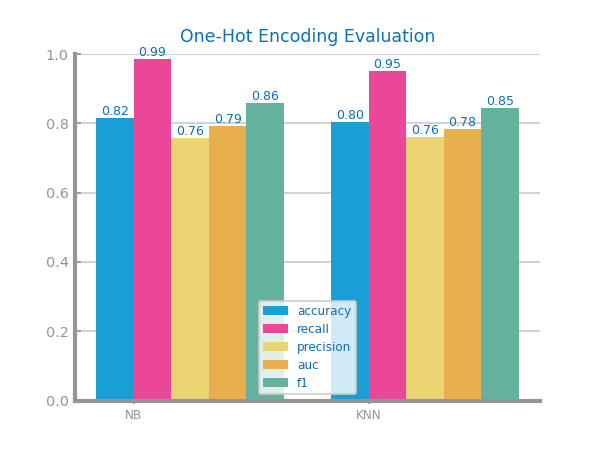
\includegraphics[width=\textwidth]{../images/lab3/traffic_accidents/1_encoding_onehot_eval.png}
    \caption{One-Hot Encoding Evaluation}
\end{subfigure}
\hfill
\begin{subfigure}{0.48\textwidth}
    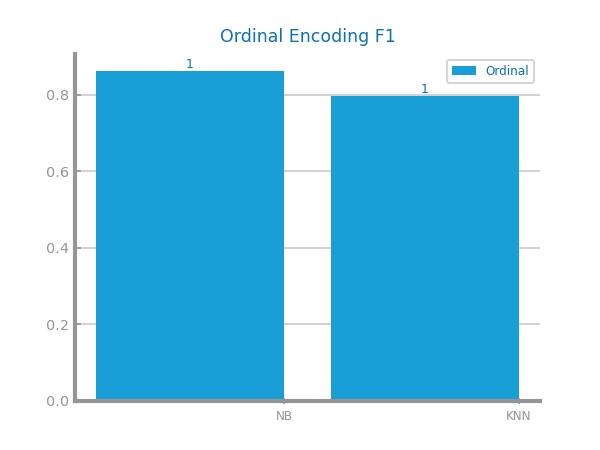
\includegraphics[width=\textwidth]{../images/lab3/traffic_accidents/1_encoding_ordinal_f1.png}
    \caption{Ordinal Encoding F1 Score}
\end{subfigure}
\caption{Detailed encoding evaluation - Traffic Accidents}
\end{figure}

\begin{figure}[H]
\centering
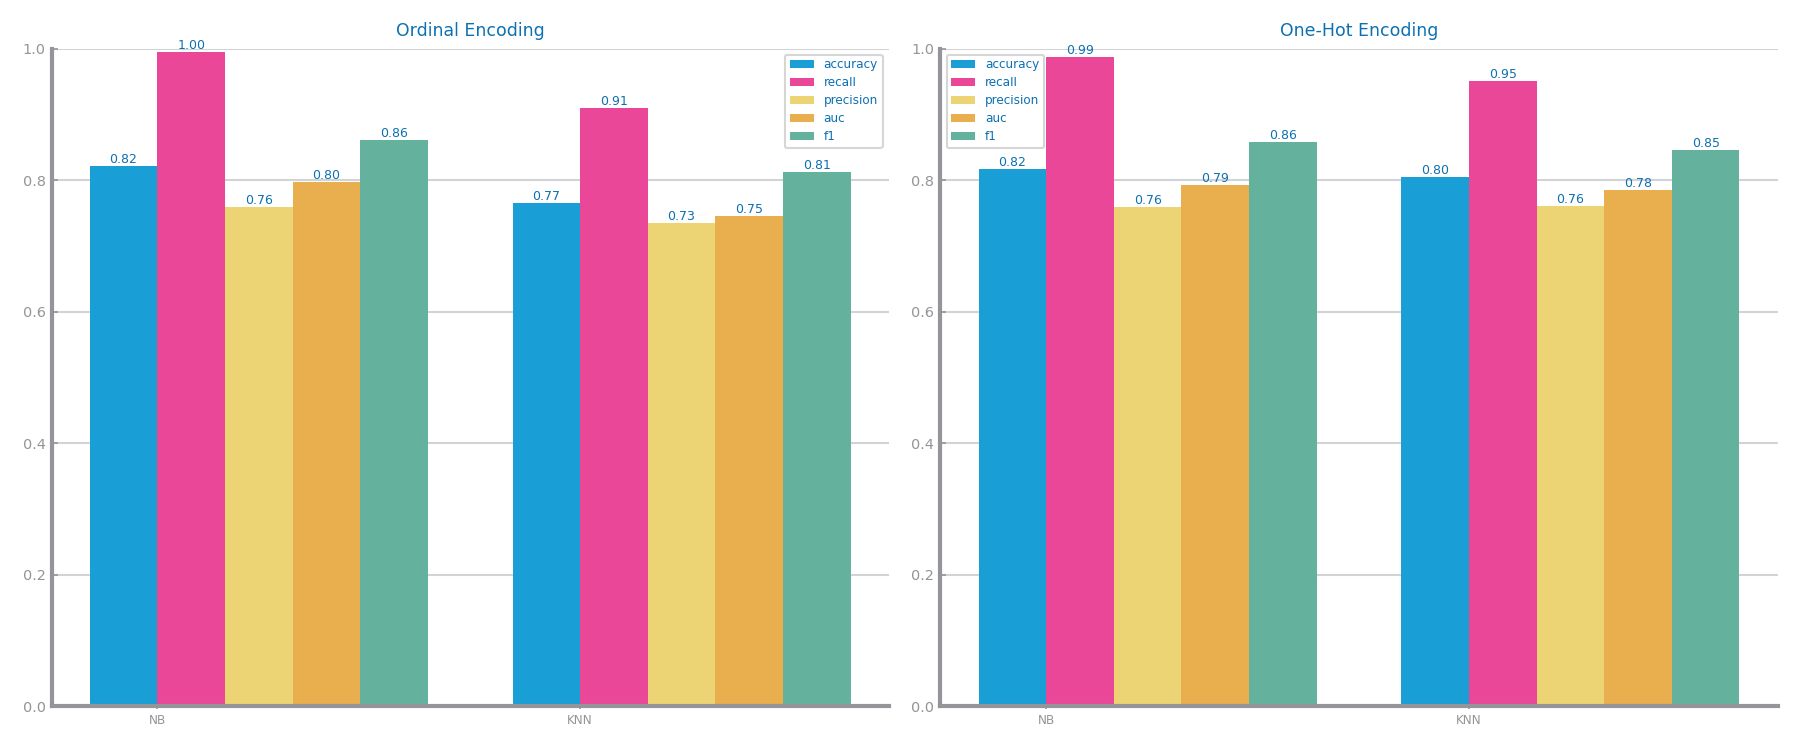
\includegraphics[width=0.85\textwidth]{../images/lab3/traffic_accidents/1_encoding_side_by_side.png}
\caption{Side-by-side encoding comparison - Traffic Accidents}
\end{figure}

\begin{figure}[H]
\centering
\begin{subfigure}{0.48\textwidth}
    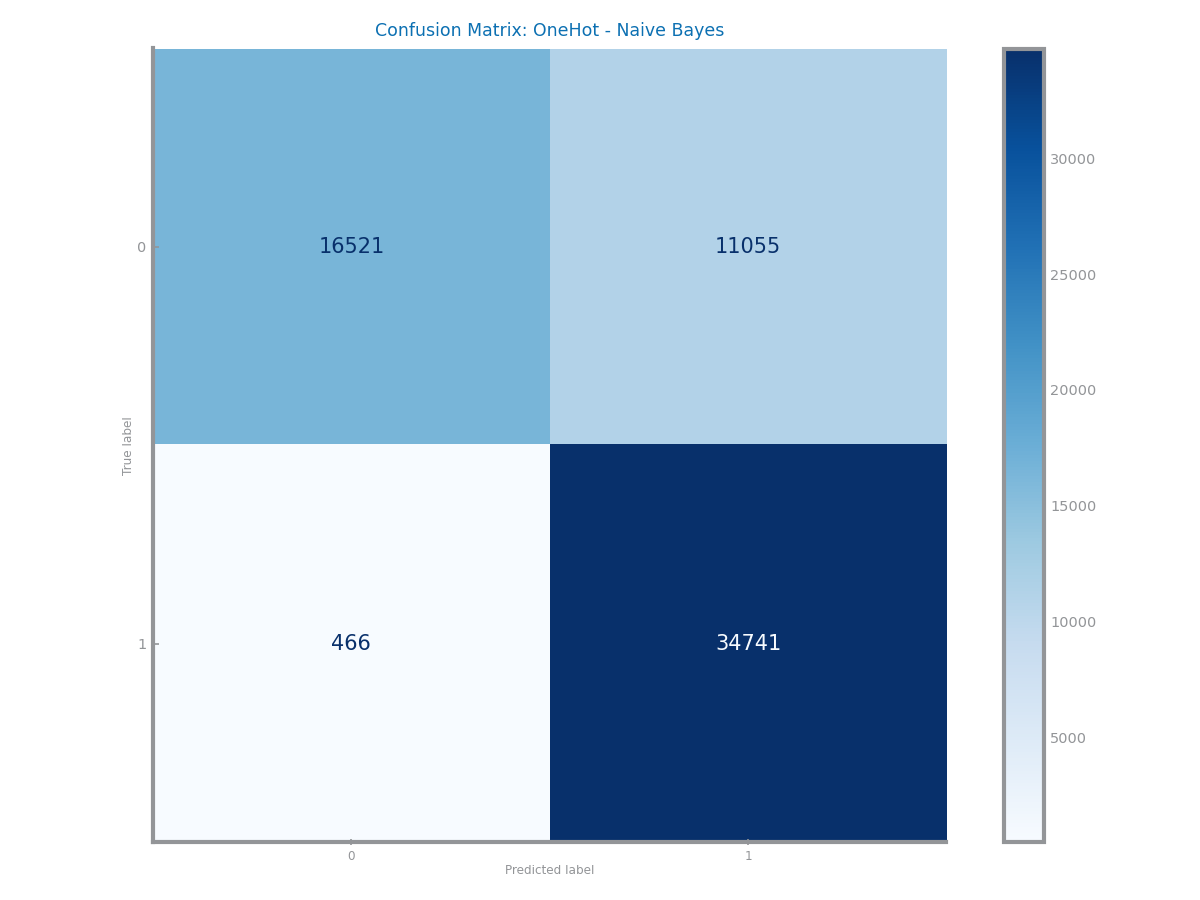
\includegraphics[width=\textwidth]{../images/lab3/traffic_accidents/1_encoding_best_nb_cm.png}
    \caption{Naive Bayes Confusion Matrix}
\end{subfigure}
\hfill
\begin{subfigure}{0.48\textwidth}
    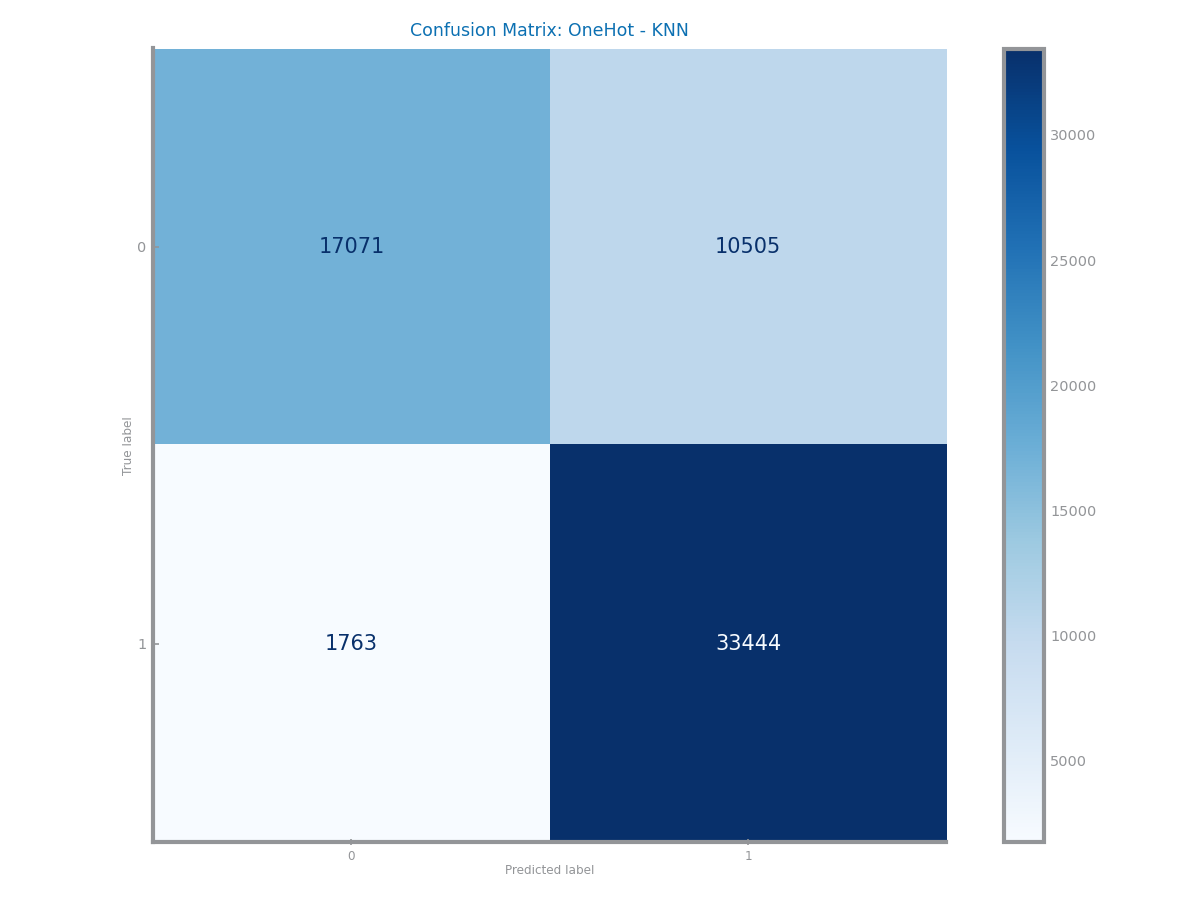
\includegraphics[width=\textwidth]{../images/lab3/traffic_accidents/1_encoding_best_knn_cm.png}
    \caption{KNN Confusion Matrix}
\end{subfigure}
\caption{Confusion matrices for best encoding approach - Traffic Accidents}
\end{figure}

% ------------------------------------------------------------
\subsection{Step 2: Missing Value Imputation}
% ------------------------------------------------------------

\begin{figure}[H]
\centering
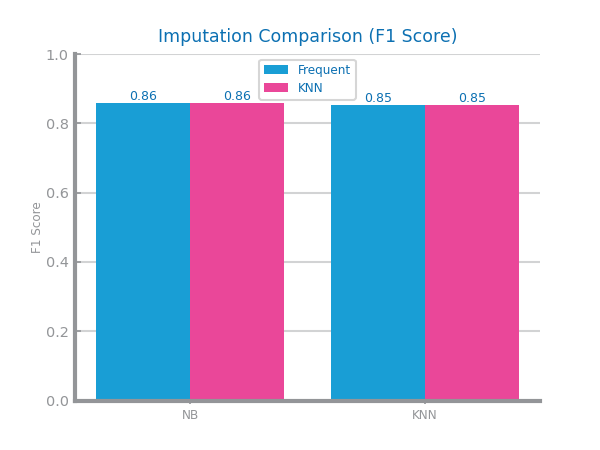
\includegraphics[width=0.85\textwidth]{../images/lab3/traffic_accidents/2_imputation_comparison.png}
\caption{Imputation approaches comparison - Traffic Accidents}
\end{figure}

\begin{figure}[H]
\centering
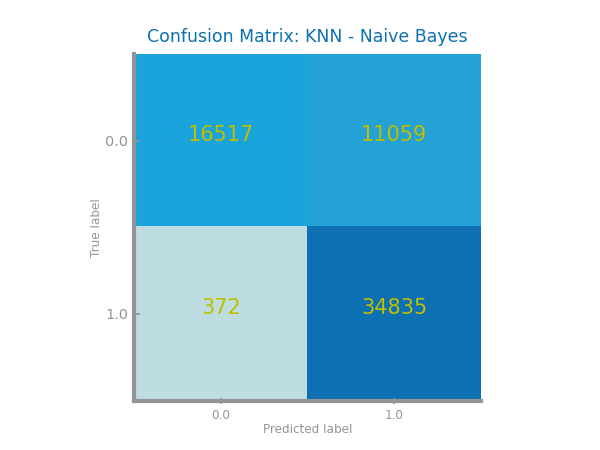
\includegraphics[width=0.6\textwidth]{../images/lab3/traffic_accidents/2_imputation_best_nb_cm.png}
\caption{Confusion matrix for best imputation approach - Traffic Accidents}
\end{figure}

% ------------------------------------------------------------
\subsection{Step 3: Outlier Treatment}
% ------------------------------------------------------------

\begin{figure}[H]
\centering
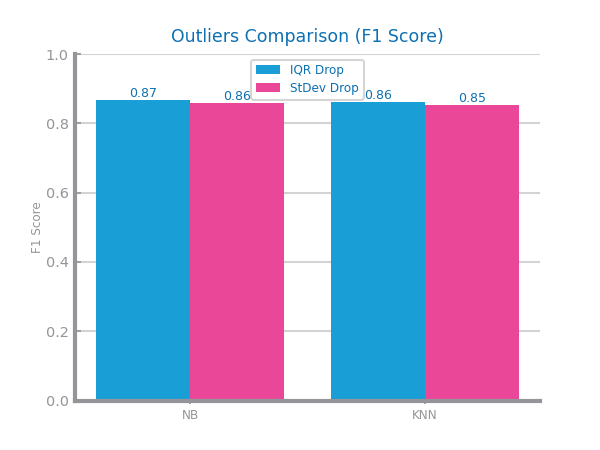
\includegraphics[width=0.85\textwidth]{../images/lab3/traffic_accidents/3_outliers_comparison.png}
\caption{Outlier treatment approaches comparison - Traffic Accidents}
\end{figure}

\begin{figure}[H]
\centering
\begin{subfigure}{0.48\textwidth}
    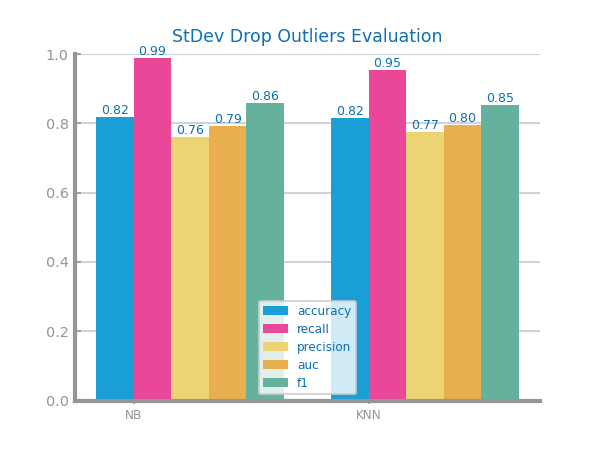
\includegraphics[width=\textwidth]{../images/lab3/traffic_accidents/3_outliers_stdev_eval.png}
    \caption{Std-based Outlier Removal}
\end{subfigure}
\hfill
\begin{subfigure}{0.48\textwidth}
    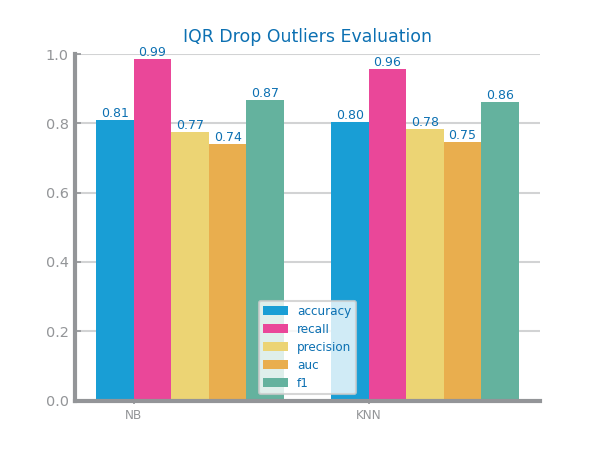
\includegraphics[width=\textwidth]{../images/lab3/traffic_accidents/3_outliers_iqr_eval.png}
    \caption{IQR-based Outlier Removal}
\end{subfigure}
\caption{Detailed outlier treatment evaluation - Traffic Accidents}
\end{figure}

\begin{figure}[H]
\centering
\begin{subfigure}{0.48\textwidth}
    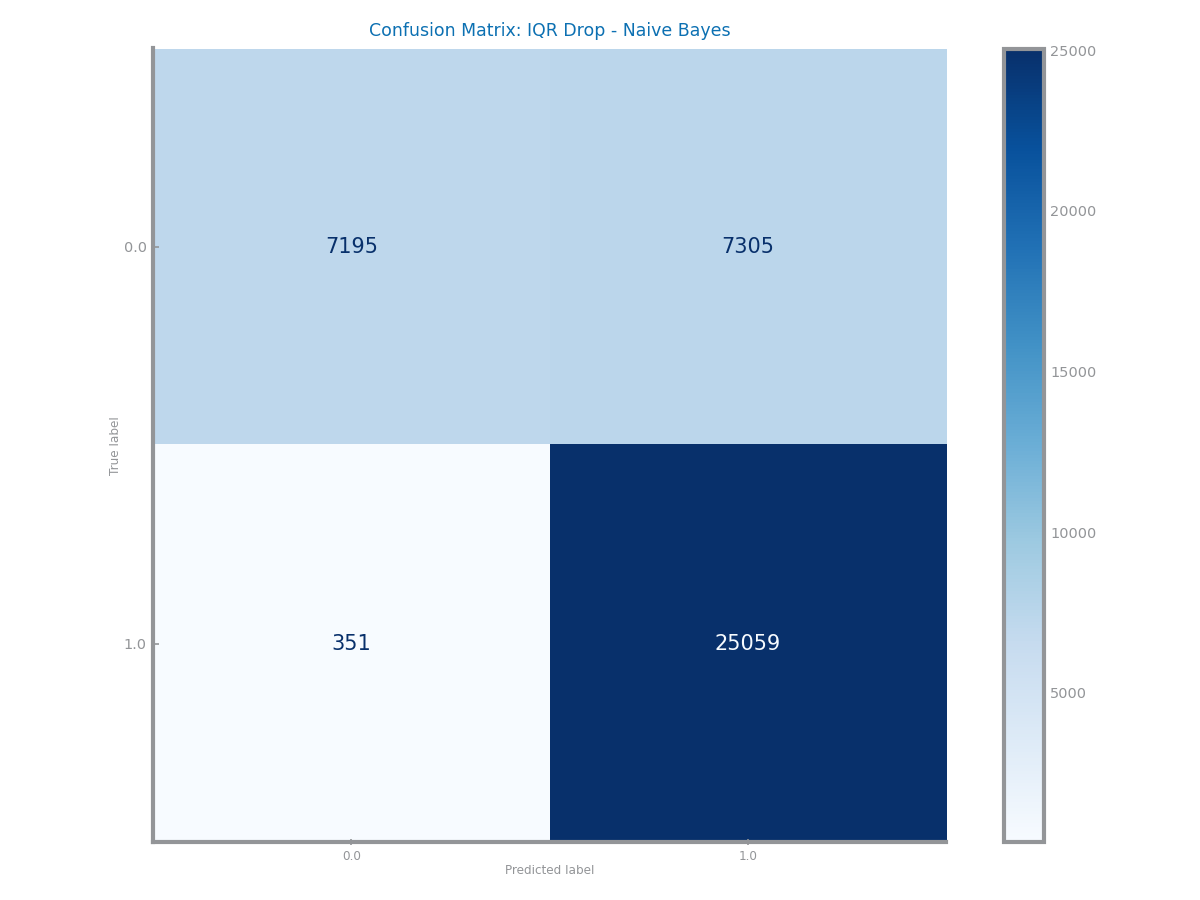
\includegraphics[width=\textwidth]{../images/lab3/traffic_accidents/3_outliers_best_nb_cm.png}
    \caption{Naive Bayes Confusion Matrix}
\end{subfigure}
\hfill
\begin{subfigure}{0.48\textwidth}
    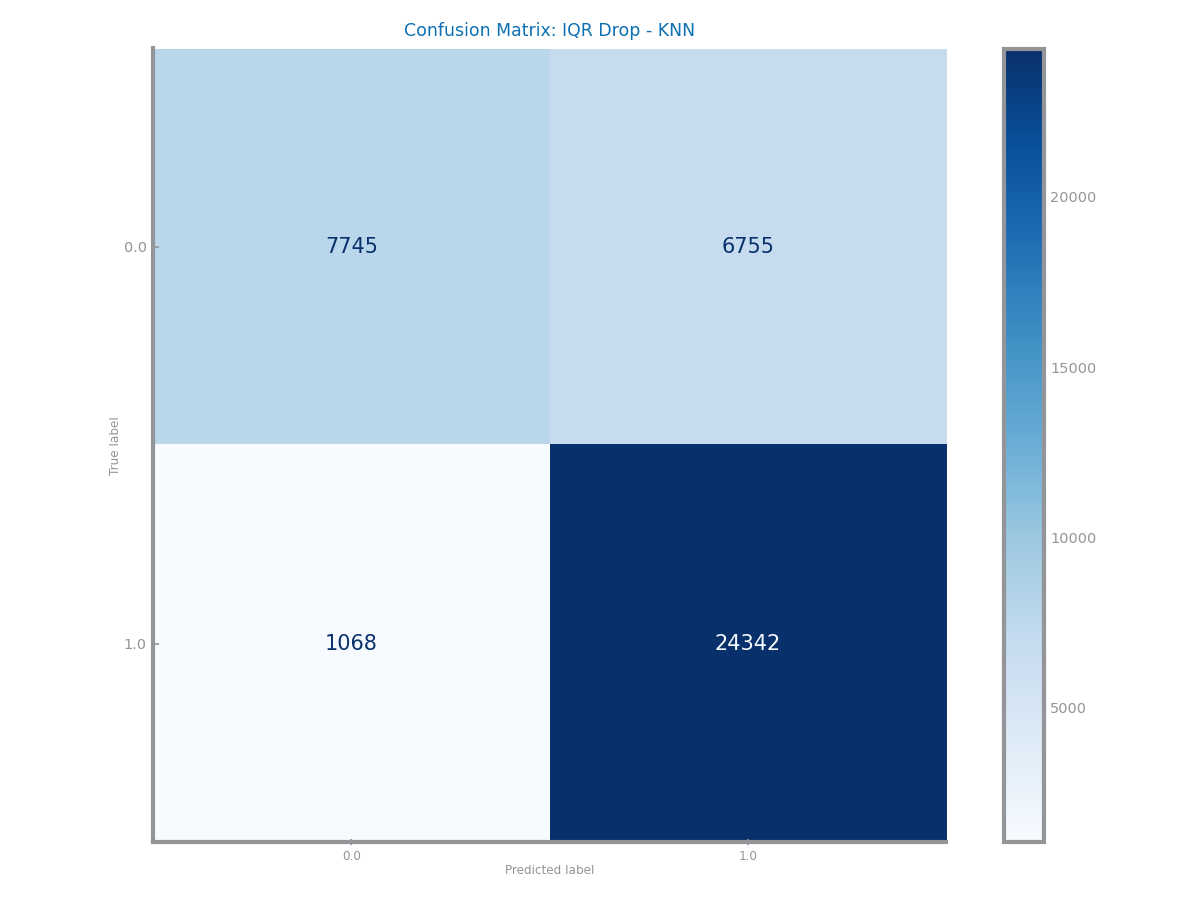
\includegraphics[width=\textwidth]{../images/lab3/traffic_accidents/3_outliers_best_knn_cm.png}
    \caption{KNN Confusion Matrix}
\end{subfigure}
\caption{Confusion matrices for best outlier treatment - Traffic Accidents}
\end{figure}

% ------------------------------------------------------------
\subsection{Step 4: Feature Scaling}
% ------------------------------------------------------------

\begin{figure}[H]
\centering
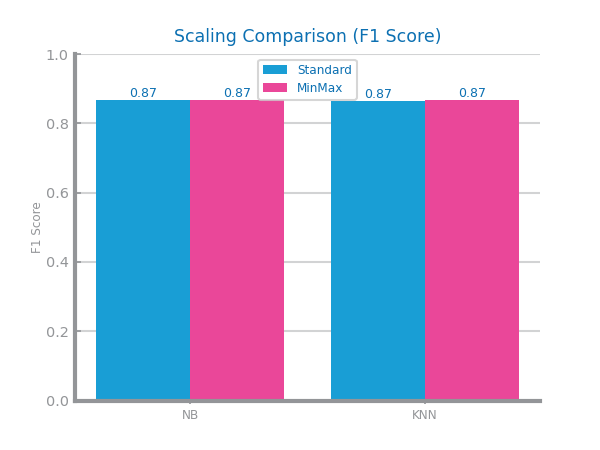
\includegraphics[width=0.85\textwidth]{../images/lab3/traffic_accidents/4_scaling_comparison.png}
\caption{Scaling approaches comparison - Traffic Accidents}
\end{figure}

\begin{figure}[H]
\centering
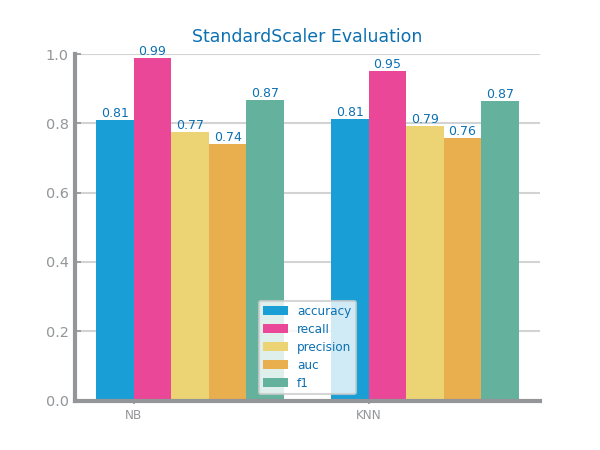
\includegraphics[width=0.75\textwidth]{../images/lab3/traffic_accidents/4_scaling_standard_eval.png}
\caption{StandardScaler evaluation - Traffic Accidents}
\end{figure}

\begin{figure}[H]
\centering
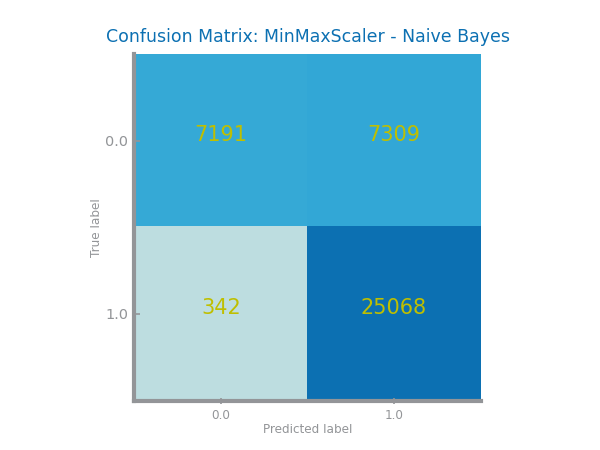
\includegraphics[width=0.6\textwidth]{../images/lab3/traffic_accidents/4_scaling_best_nb_cm.png}
\caption{Confusion matrix for best scaling approach - Traffic Accidents}
\end{figure}

% ------------------------------------------------------------
\subsection{Step 5: Class Balancing}
% ------------------------------------------------------------

\begin{figure}[H]
\centering
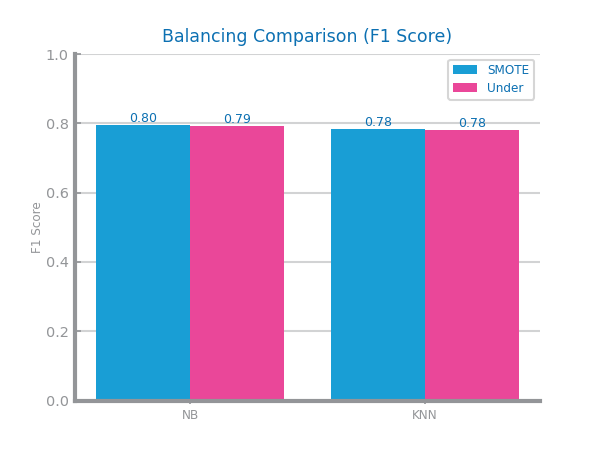
\includegraphics[width=0.85\textwidth]{../images/lab3/traffic_accidents/5_balancing_comparison.png}
\caption{Balancing approaches comparison - Traffic Accidents}
\end{figure}

\begin{figure}[H]
\centering
\begin{subfigure}{0.48\textwidth}
    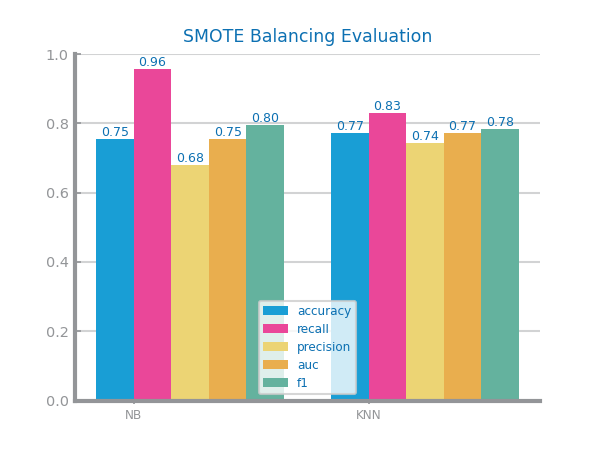
\includegraphics[width=\textwidth]{../images/lab3/traffic_accidents/5_balancing_smote_eval.png}
    \caption{SMOTE Evaluation}
\end{subfigure}
\hfill
\begin{subfigure}{0.48\textwidth}
    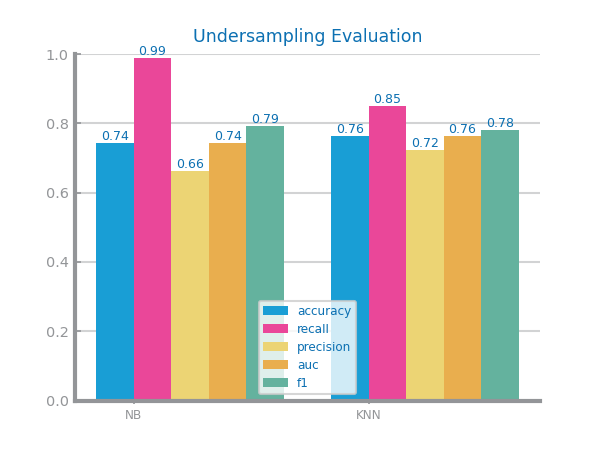
\includegraphics[width=\textwidth]{../images/lab3/traffic_accidents/5_balancing_under_eval.png}
    \caption{Undersampling Evaluation}
\end{subfigure}
\caption{Detailed balancing evaluation - Traffic Accidents}
\end{figure}

\begin{figure}[H]
\centering
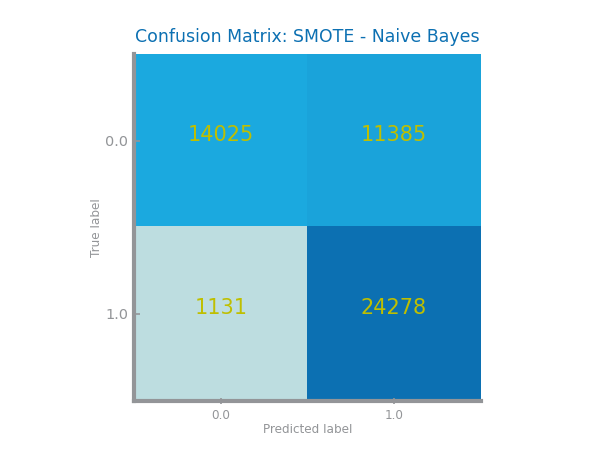
\includegraphics[width=0.6\textwidth]{../images/lab3/traffic_accidents/5_balancing_best_nb_cm.png}
\caption{Confusion matrix for best balancing approach - Traffic Accidents}
\end{figure}

% ------------------------------------------------------------
\subsection{Step 6: Feature Selection}
% ------------------------------------------------------------

\begin{figure}[H]
\centering
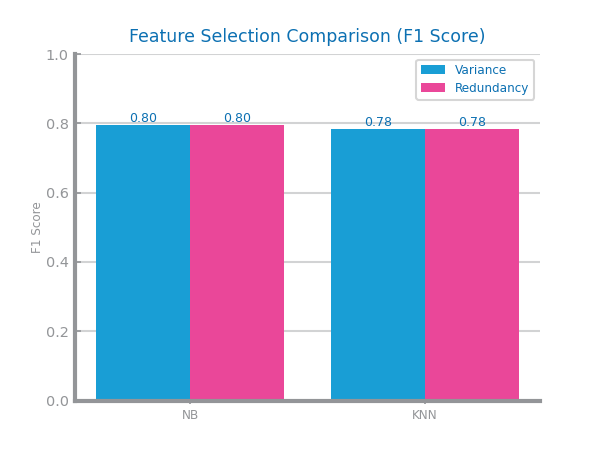
\includegraphics[width=0.85\textwidth]{../images/lab3/traffic_accidents/6_selection_comparison.png}
\caption{Feature selection approaches comparison - Traffic Accidents}
\end{figure}

\begin{figure}[H]
\centering
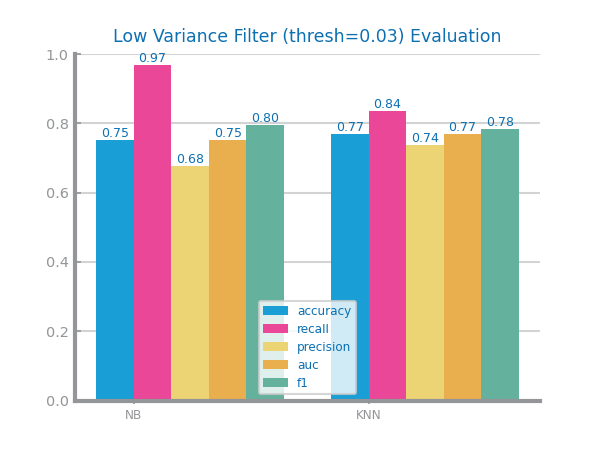
\includegraphics[width=0.75\textwidth]{../images/lab3/traffic_accidents/6_selection_variance_eval.png}
\caption{Variance threshold evaluation - Traffic Accidents}
\end{figure}

\begin{figure}[H]
\centering
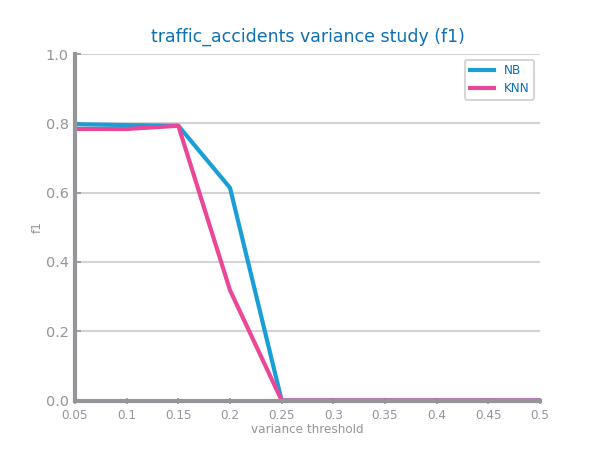
\includegraphics[width=0.85\textwidth]{../images/lab3/traffic_accidents/6_selection_variance_f1.png}
\caption{Variance study for feature selection - Traffic Accidents}
\end{figure}

\begin{figure}[H]
\centering
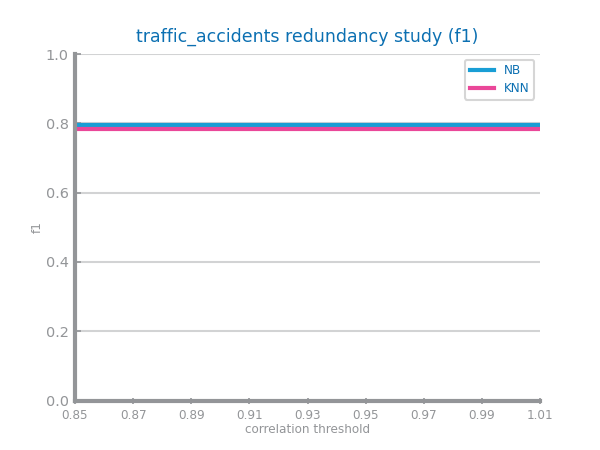
\includegraphics[width=0.85\textwidth]{../images/lab3/traffic_accidents/6_selection_redundancy_f1.png}
\caption{Redundancy study for feature selection - Traffic Accidents}
\end{figure}

\clearpage

% ============================================================
\section{Flights Dataset}
% ============================================================

% ------------------------------------------------------------
\subsection{Step 1: Variable Encoding}
% ------------------------------------------------------------

\begin{figure}[H]
\centering
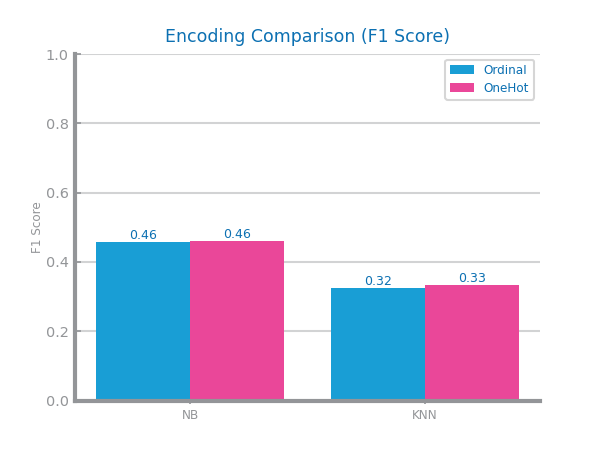
\includegraphics[width=0.85\textwidth]{../images/lab3/flights/1_encoding_comparison.png}
\caption{Encoding approaches comparison - Flights}
\end{figure}

\begin{figure}[H]
\centering
\begin{subfigure}{0.48\textwidth}
    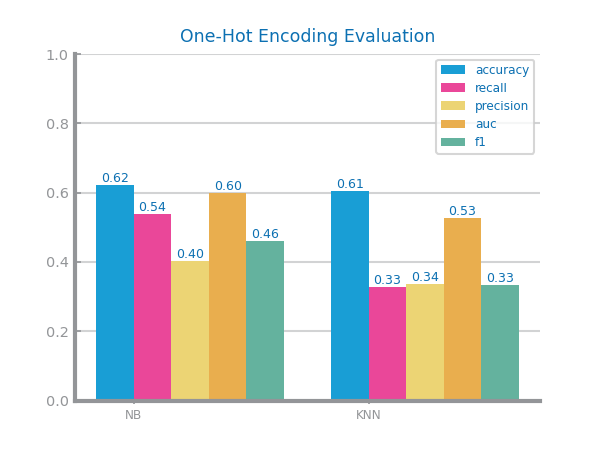
\includegraphics[width=\textwidth]{../images/lab3/flights/1_encoding_onehot_eval.png}
    \caption{One-Hot Encoding Evaluation}
\end{subfigure}
\hfill
\begin{subfigure}{0.48\textwidth}
    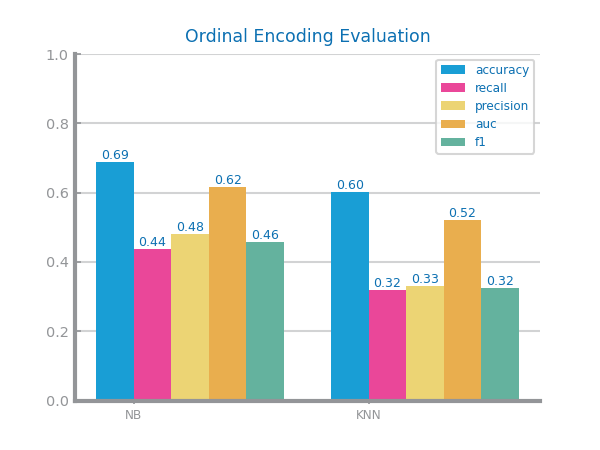
\includegraphics[width=\textwidth]{../images/lab3/flights/1_encoding_ordinal_eval.png}
    \caption{Ordinal Encoding Evaluation}
\end{subfigure}
\caption{Detailed encoding evaluation - Flights}
\end{figure}

\begin{figure}[H]
\centering
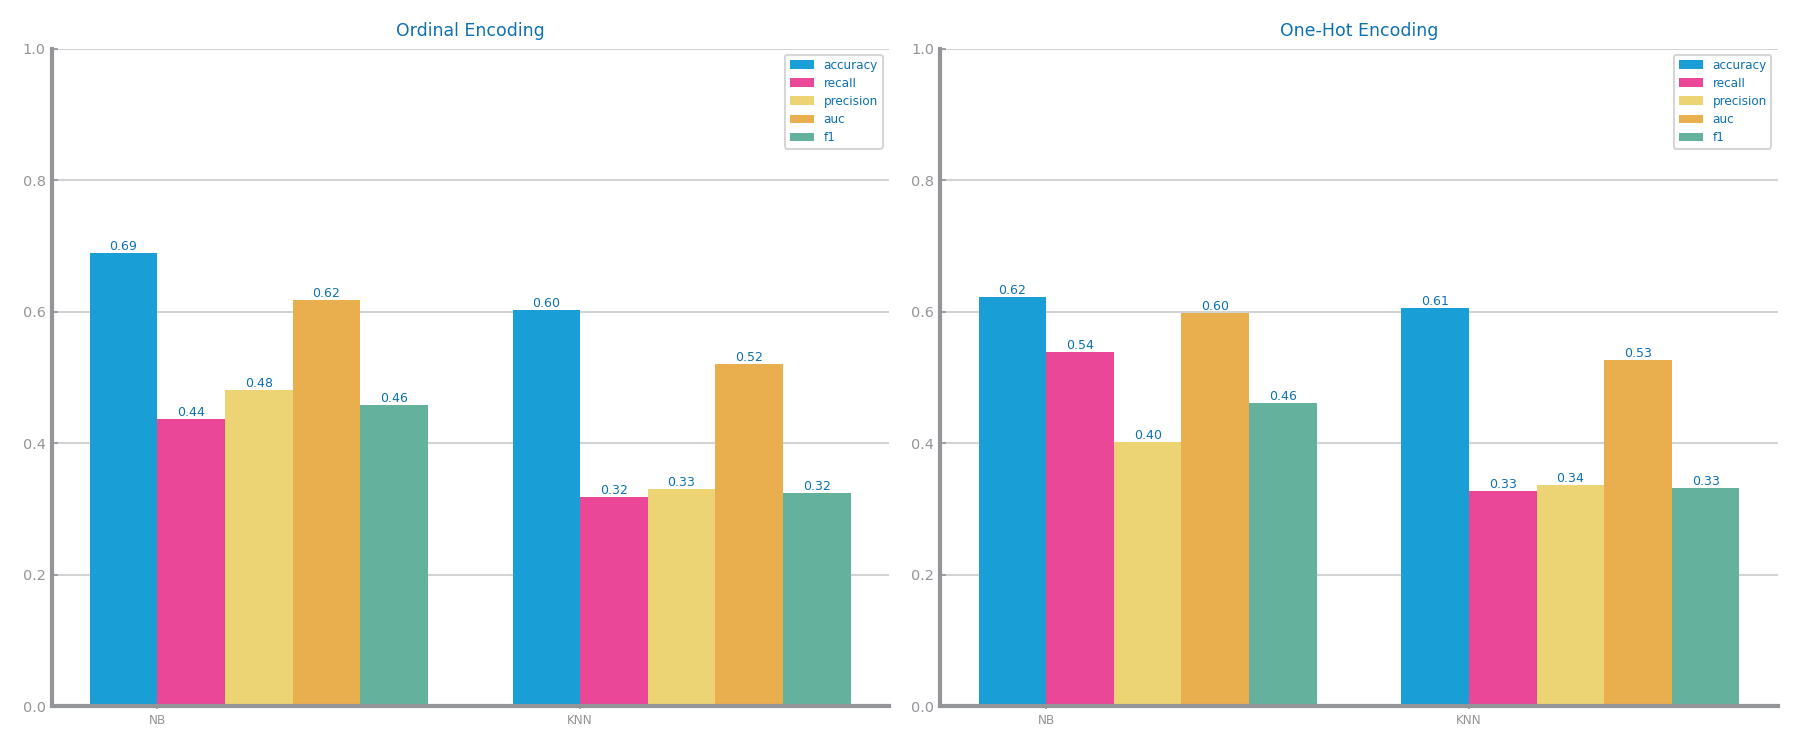
\includegraphics[width=0.85\textwidth]{../images/lab3/flights/1_encoding_side_by_side.png}
\caption{Side-by-side encoding comparison - Flights}
\end{figure}

\begin{figure}[H]
\centering
\begin{subfigure}{0.48\textwidth}
    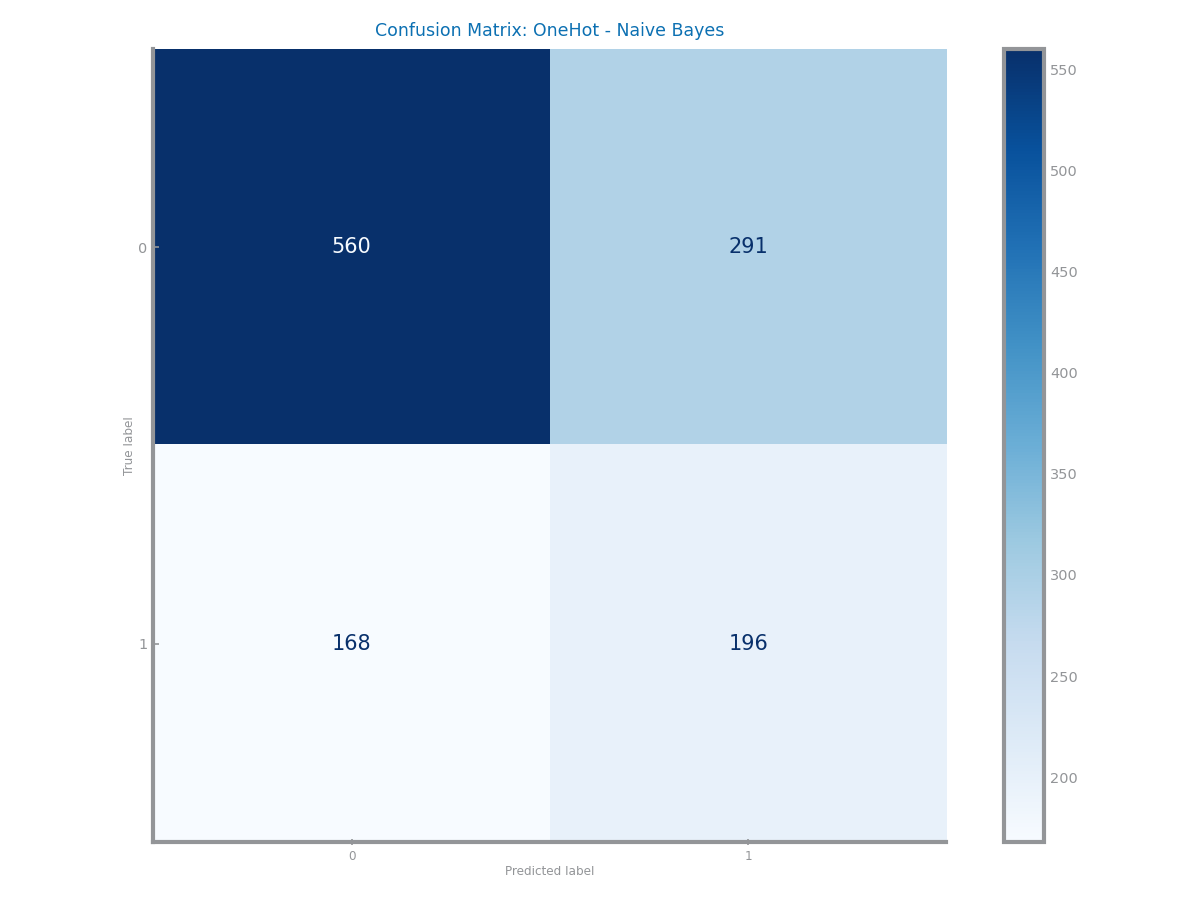
\includegraphics[width=\textwidth]{../images/lab3/flights/1_encoding_best_nb_cm.png}
    \caption{Naive Bayes Confusion Matrix}
\end{subfigure}
\hfill
\begin{subfigure}{0.48\textwidth}
    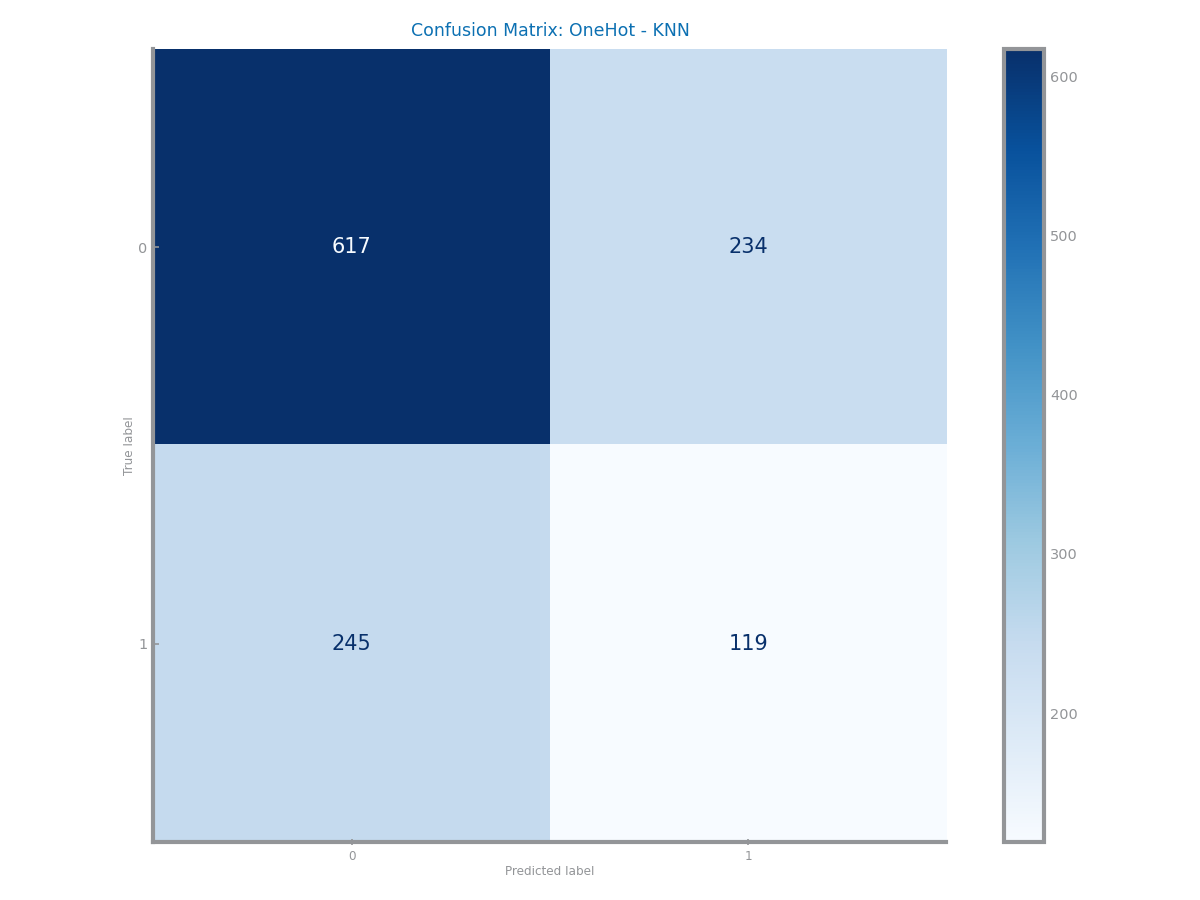
\includegraphics[width=\textwidth]{../images/lab3/flights/1_encoding_best_knn_cm.png}
    \caption{KNN Confusion Matrix}
\end{subfigure}
\caption{Confusion matrices for best encoding approach - Flights}
\end{figure}

% ------------------------------------------------------------
\subsection{Step 3: Outlier Treatment}
% ------------------------------------------------------------

\begin{figure}[H]
\centering
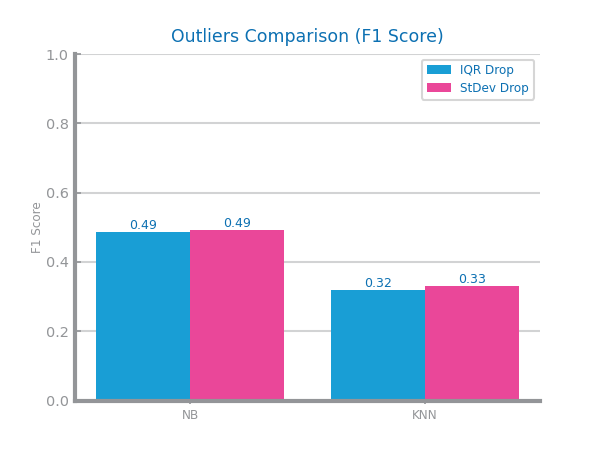
\includegraphics[width=0.85\textwidth]{../images/lab3/flights/3_outliers_comparison.png}
\caption{Outlier treatment approaches comparison - Flights}
\end{figure}

\begin{figure}[H]
\centering
\begin{subfigure}{0.48\textwidth}
    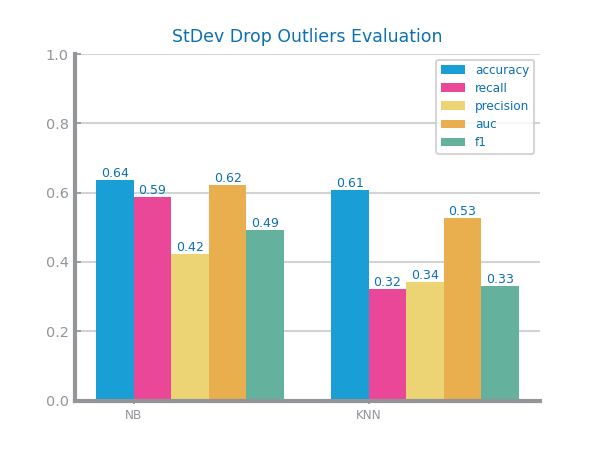
\includegraphics[width=\textwidth]{../images/lab3/flights/3_outliers_stdev_eval.png}
    \caption{Std-based Outlier Removal}
\end{subfigure}
\hfill
\begin{subfigure}{0.48\textwidth}
    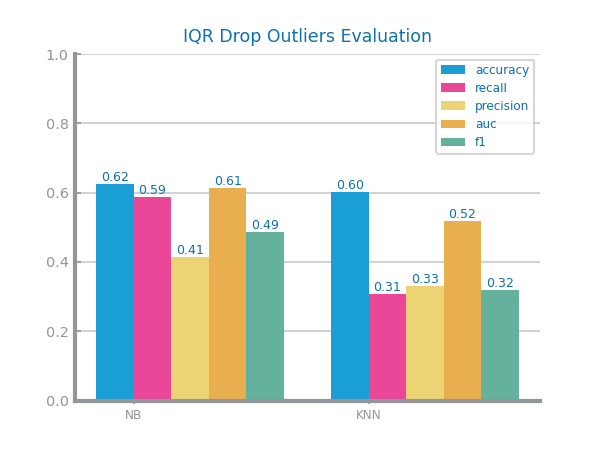
\includegraphics[width=\textwidth]{../images/lab3/flights/3_outliers_iqr_eval.png}
    \caption{IQR-based Outlier Removal}
\end{subfigure}
\caption{Detailed outlier treatment evaluation - Flights}
\end{figure}

\begin{figure}[H]
\centering
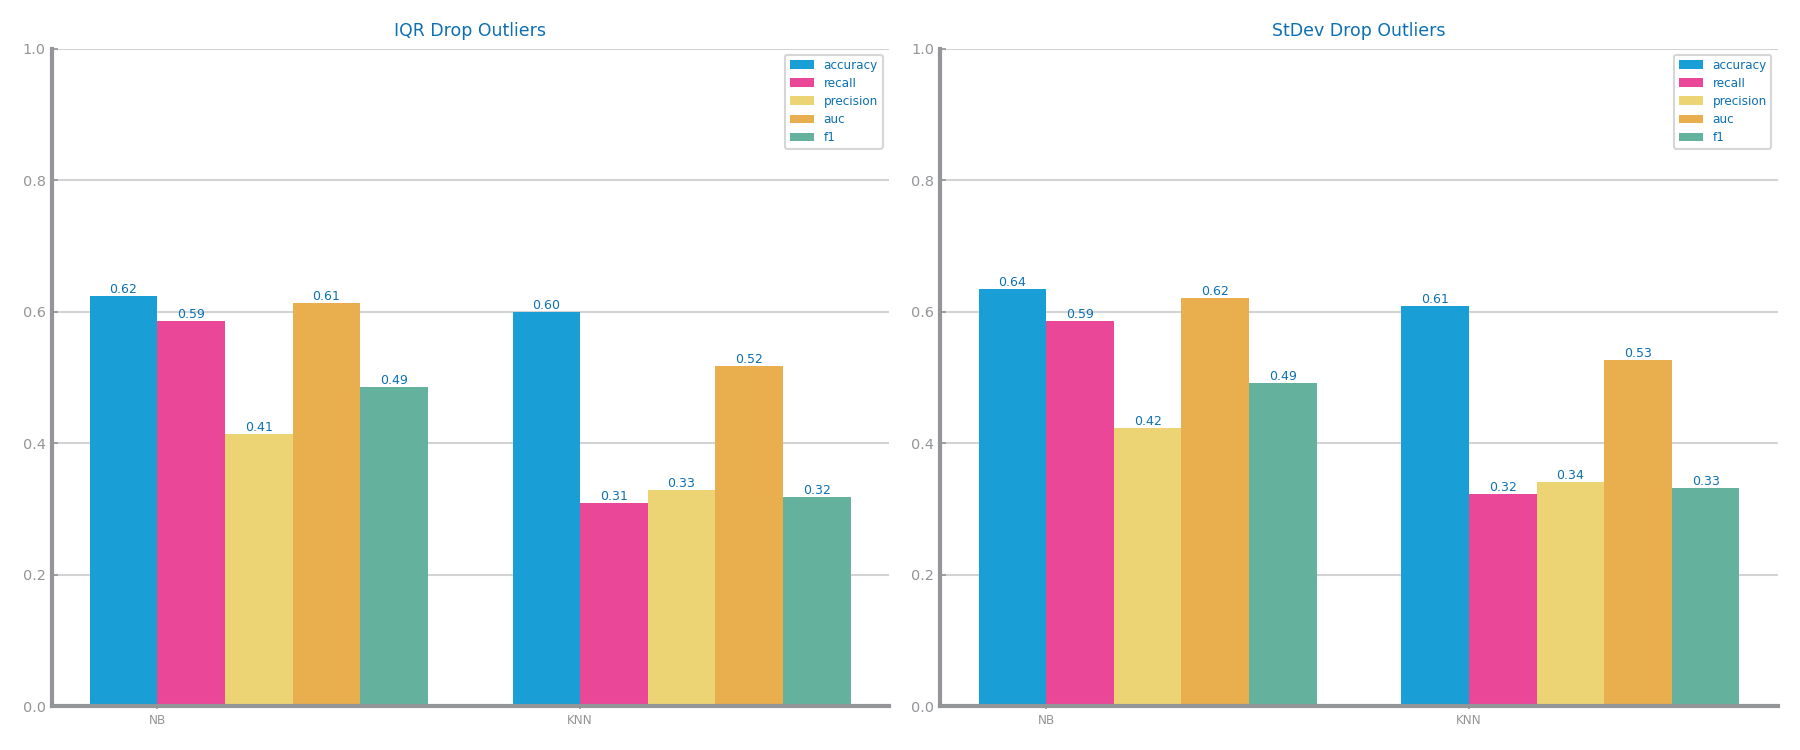
\includegraphics[width=0.85\textwidth]{../images/lab3/flights/3_outliers_side_by_side.png}
\caption{Side-by-side outlier treatment comparison - Flights}
\end{figure}

\begin{figure}[H]
\centering
\begin{subfigure}{0.48\textwidth}
    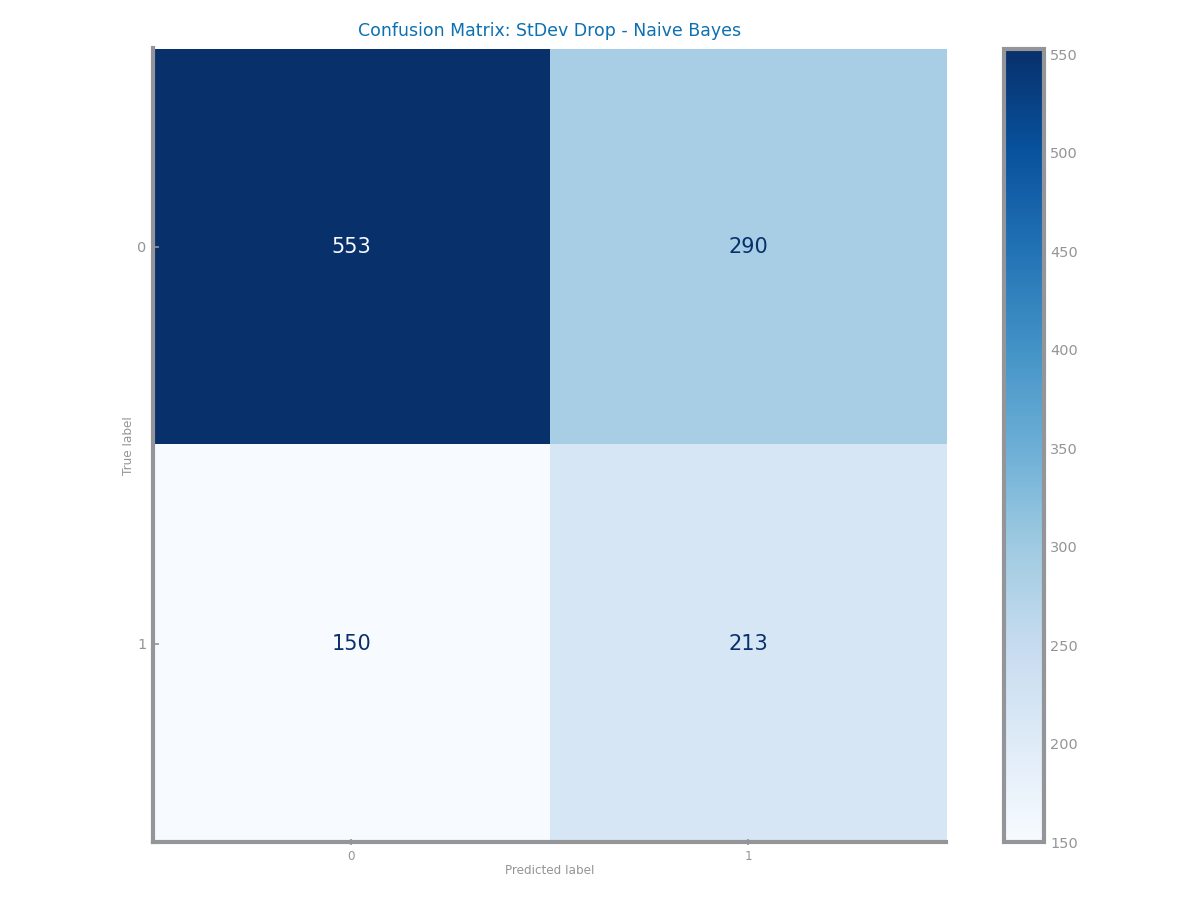
\includegraphics[width=\textwidth]{../images/lab3/flights/3_outliers_best_nb_cm.png}
    \caption{Naive Bayes Confusion Matrix}
\end{subfigure}
\hfill
\begin{subfigure}{0.48\textwidth}
    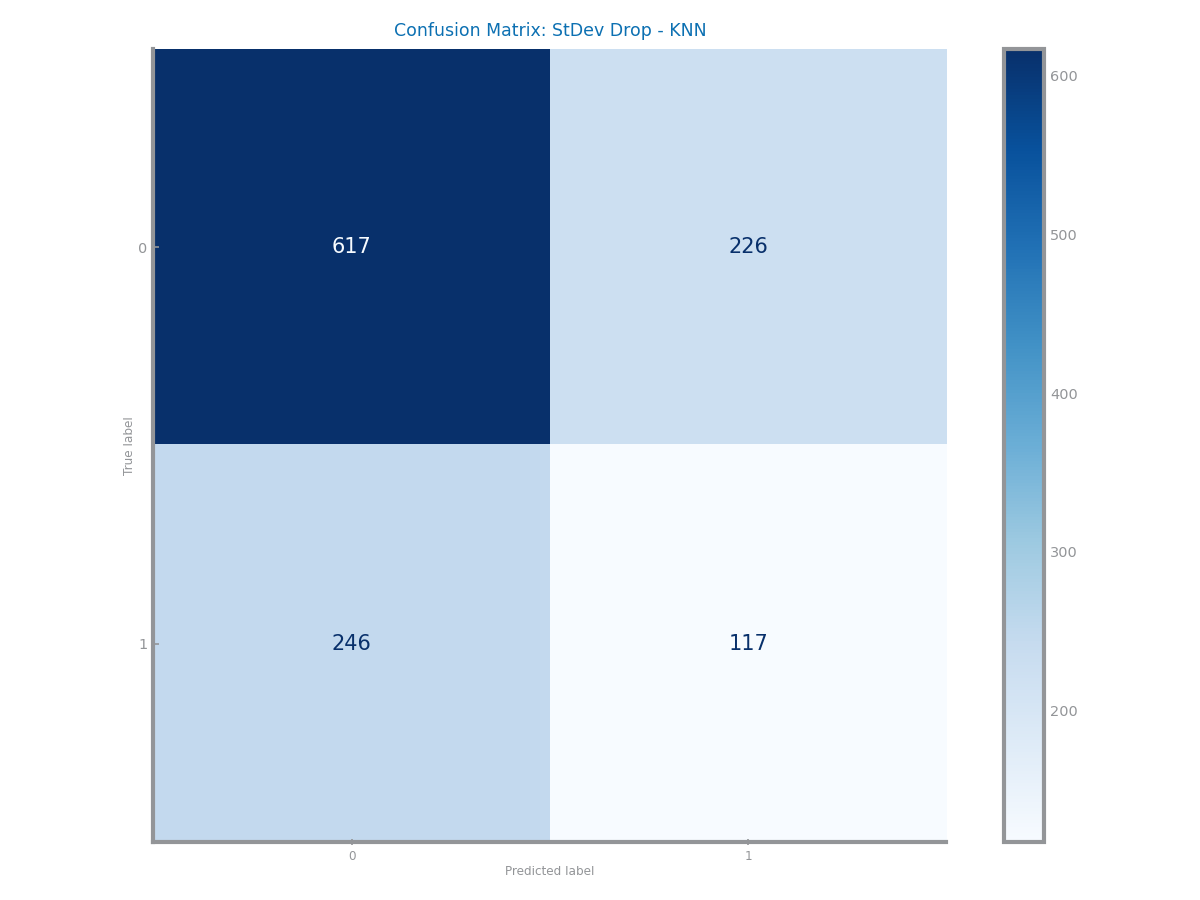
\includegraphics[width=\textwidth]{../images/lab3/flights/3_outliers_best_knn_cm.png}
    \caption{KNN Confusion Matrix}
\end{subfigure}
\caption{Confusion matrices for best outlier treatment - Flights}
\end{figure}

% ------------------------------------------------------------
\subsection{Step 4: Feature Scaling}
% ------------------------------------------------------------

\begin{figure}[H]
\centering
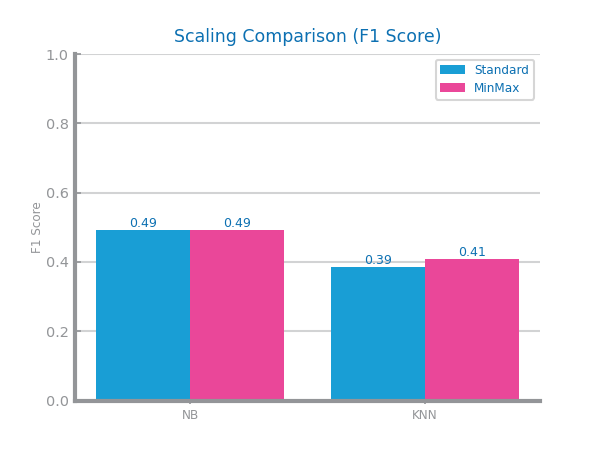
\includegraphics[width=0.85\textwidth]{../images/lab3/flights/4_scaling_comparison.png}
\caption{Scaling approaches comparison - Flights}
\end{figure}

\begin{figure}[H]
\centering
\begin{subfigure}{0.48\textwidth}
    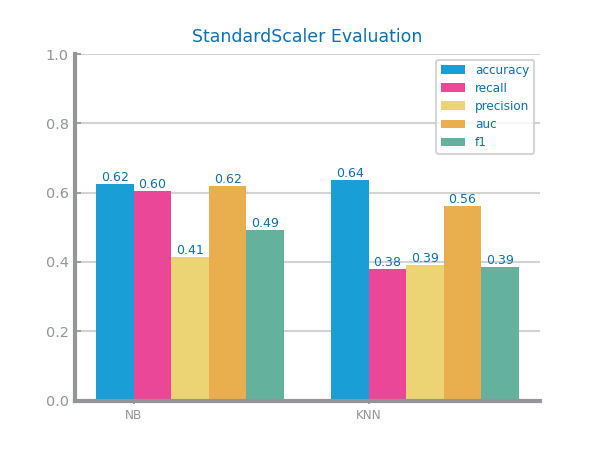
\includegraphics[width=\textwidth]{../images/lab3/flights/4_scaling_standard_eval.png}
    \caption{StandardScaler Evaluation}
\end{subfigure}
\hfill
\begin{subfigure}{0.48\textwidth}
    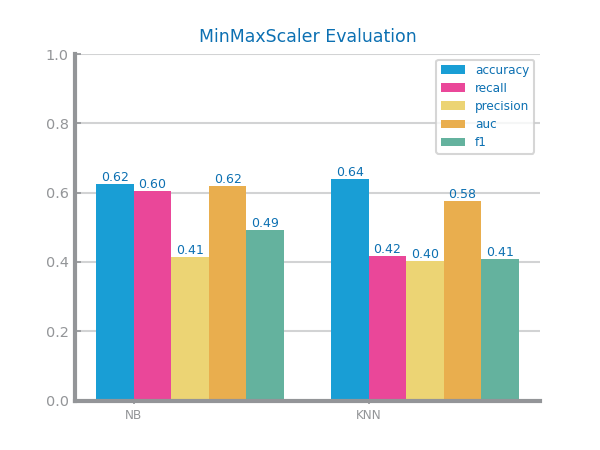
\includegraphics[width=\textwidth]{../images/lab3/flights/4_scaling_minmax_eval.png}
    \caption{MinMaxScaler Evaluation}
\end{subfigure}
\caption{Detailed scaling evaluation - Flights}
\end{figure}

\begin{figure}[H]
\centering
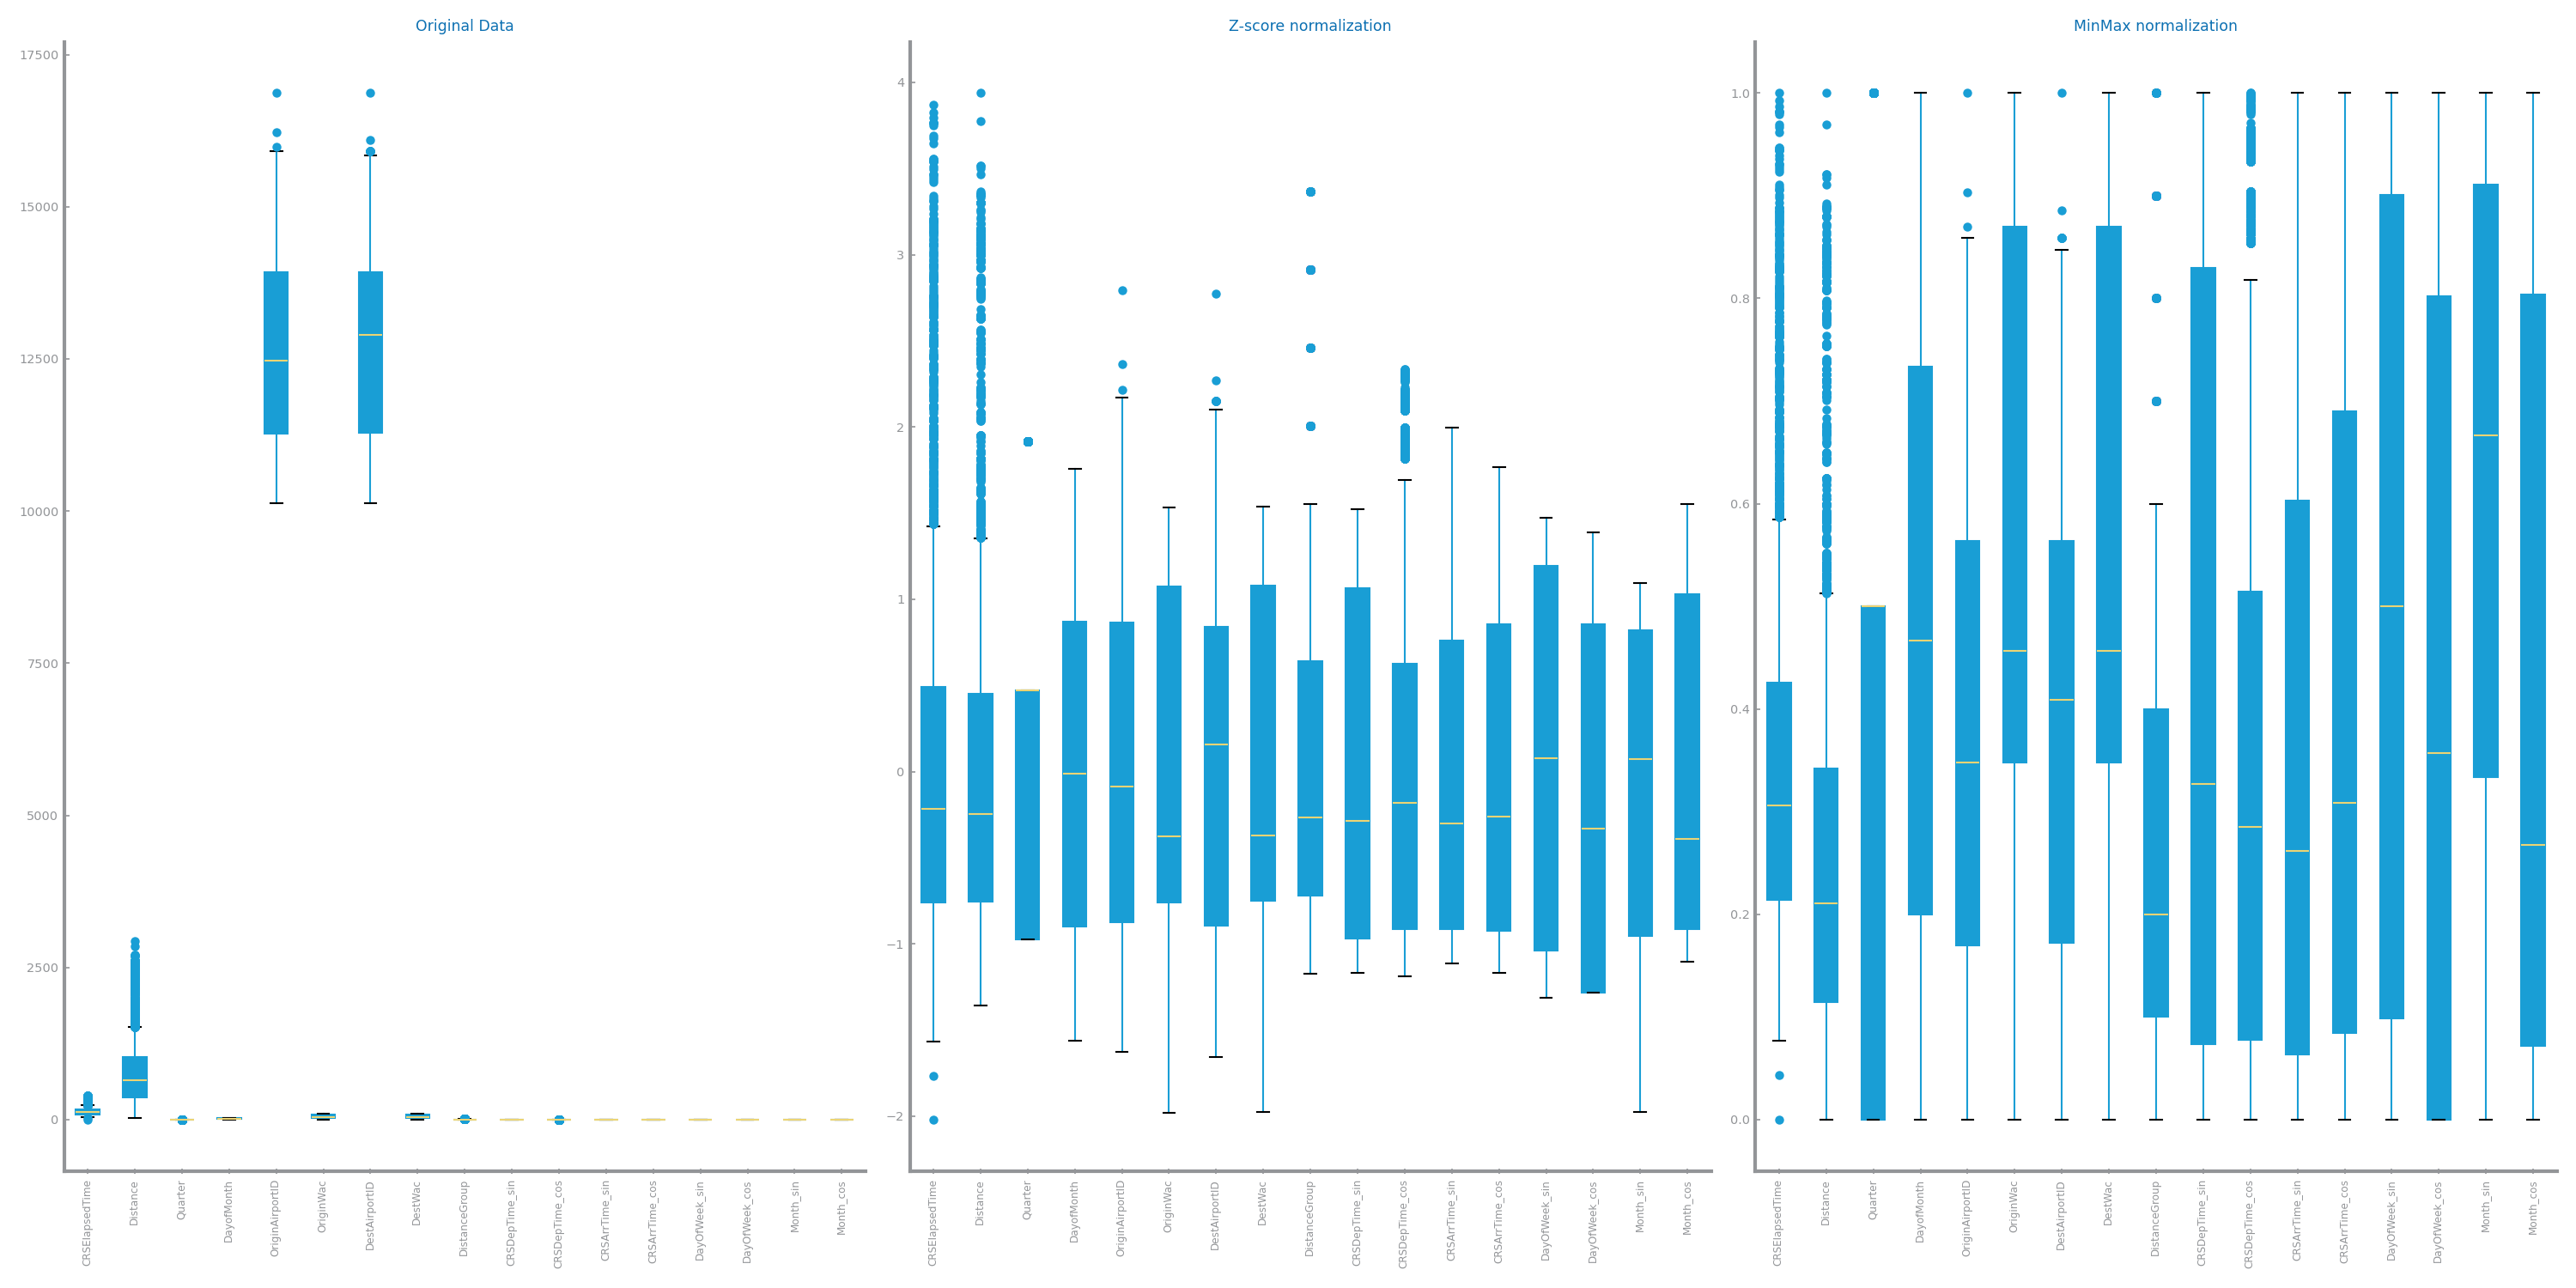
\includegraphics[width=0.85\textwidth]{../images/lab3/flights/4_scaling_boxplots.png}
\caption{Boxplots after scaling - Flights}
\end{figure}

\begin{figure}[H]
\centering
\begin{subfigure}{0.48\textwidth}
    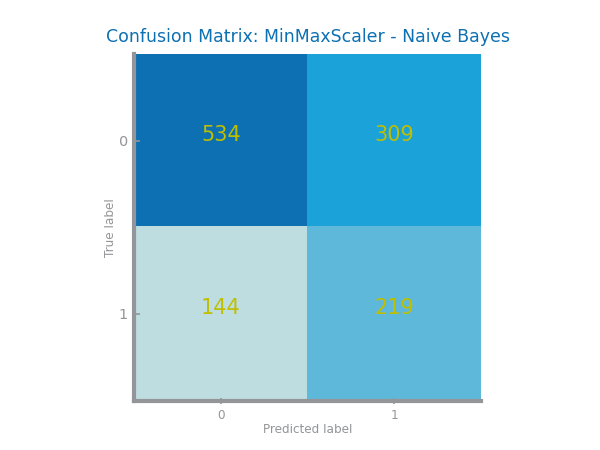
\includegraphics[width=\textwidth]{../images/lab3/flights/4_scaling_best_nb_cm.png}
    \caption{Naive Bayes Confusion Matrix}
\end{subfigure}
\hfill
\begin{subfigure}{0.48\textwidth}
    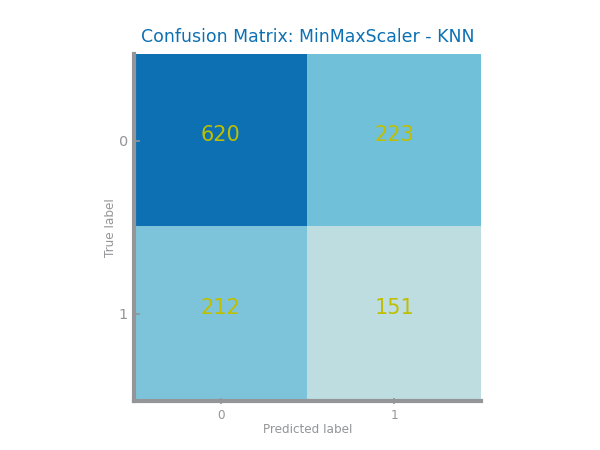
\includegraphics[width=\textwidth]{../images/lab3/flights/4_scaling_best_knn_cm.png}
    \caption{KNN Confusion Matrix}
\end{subfigure}
\caption{Confusion matrices for best scaling approach - Flights}
\end{figure}

% ------------------------------------------------------------
\subsection{Step 5: Class Balancing}
% ------------------------------------------------------------

\begin{figure}[H]
\centering
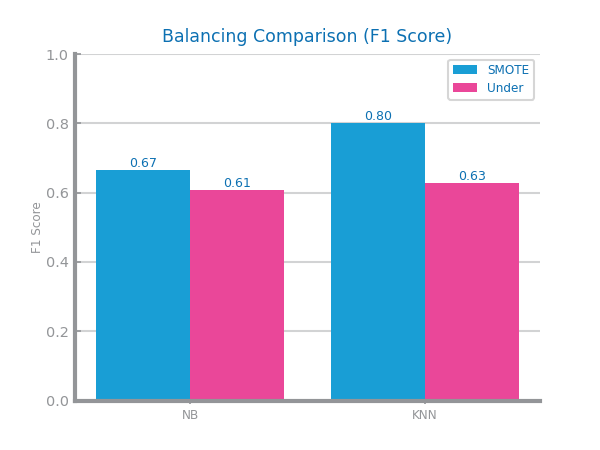
\includegraphics[width=0.85\textwidth]{../images/lab3/flights/5_balancing_comparison.png}
\caption{Balancing approaches comparison - Flights}
\end{figure}

\begin{figure}[H]
\centering
\begin{subfigure}{0.48\textwidth}
    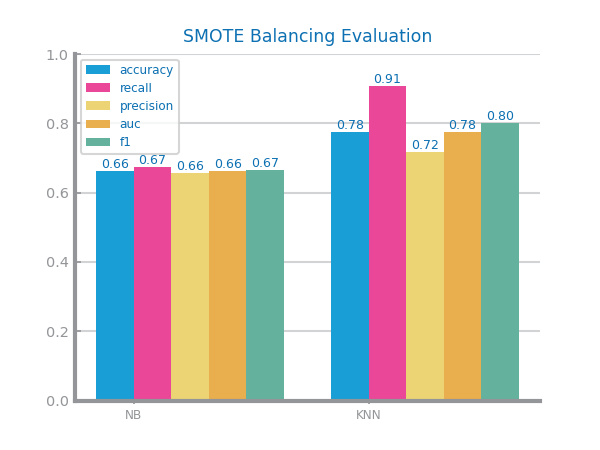
\includegraphics[width=\textwidth]{../images/lab3/flights/5_balancing_smote_eval.png}
    \caption{SMOTE Evaluation}
\end{subfigure}
\hfill
\begin{subfigure}{0.48\textwidth}
    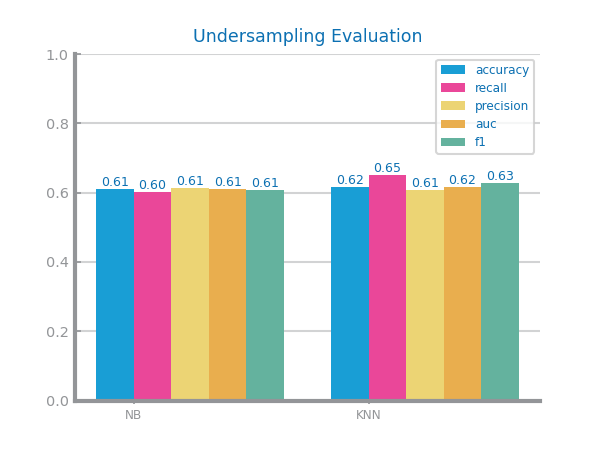
\includegraphics[width=\textwidth]{../images/lab3/flights/5_balancing_under_eval.png}
    \caption{Undersampling Evaluation}
\end{subfigure}
\caption{Detailed balancing evaluation - Flights}
\end{figure}

\begin{figure}[H]
\centering
\begin{subfigure}{0.48\textwidth}
    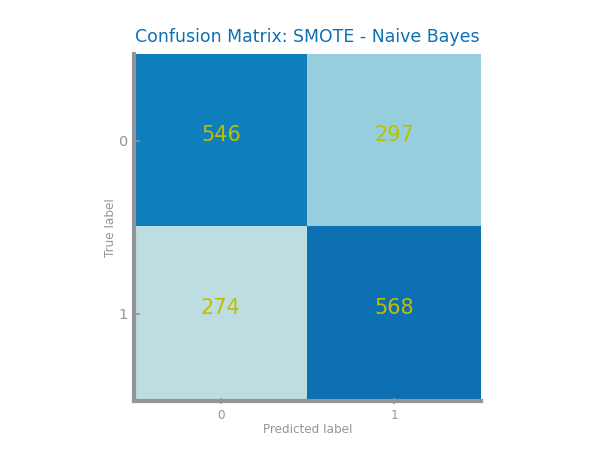
\includegraphics[width=\textwidth]{../images/lab3/flights/5_balancing_best_nb_cm.png}
    \caption{Naive Bayes Confusion Matrix}
\end{subfigure}
\hfill
\begin{subfigure}{0.48\textwidth}
    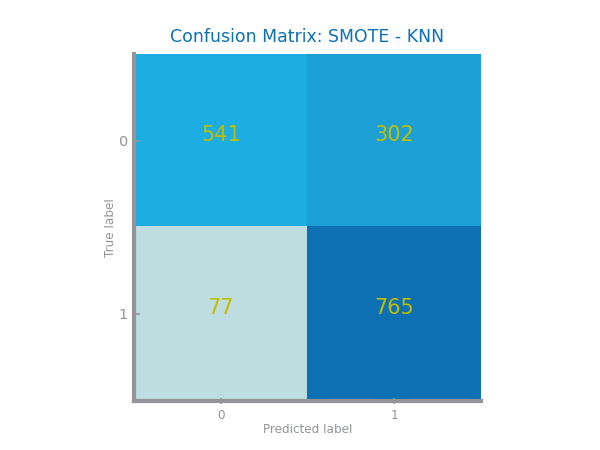
\includegraphics[width=\textwidth]{../images/lab3/flights/5_balancing_best_knn_cm.png}
    \caption{KNN Confusion Matrix}
\end{subfigure}
\caption{Confusion matrices for best balancing approach - Flights}
\end{figure}

% ------------------------------------------------------------
\subsection{Step 6: Feature Selection}
% ------------------------------------------------------------

\begin{figure}[H]
\centering
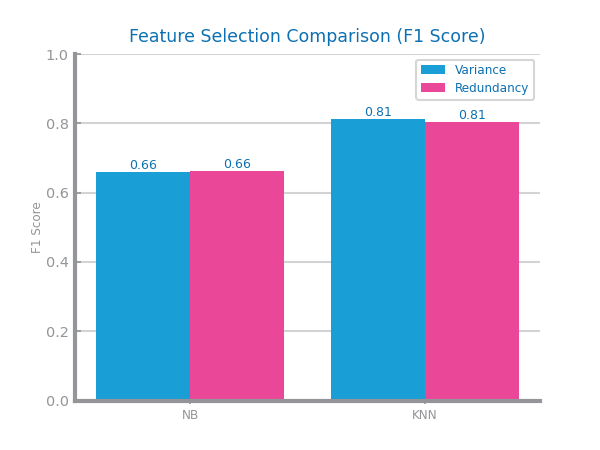
\includegraphics[width=0.85\textwidth]{../images/lab3/flights/6_selection_comparison.png}
\caption{Feature selection approaches comparison - Flights}
\end{figure}

\begin{figure}[H]
\centering
\begin{subfigure}{0.48\textwidth}
    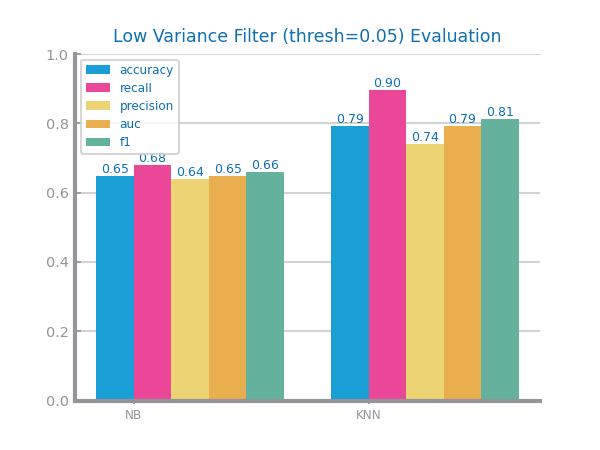
\includegraphics[width=\textwidth]{../images/lab3/flights/6_selection_variance_eval.png}
    \caption{Variance Threshold Evaluation}
\end{subfigure}
\hfill
\begin{subfigure}{0.48\textwidth}
    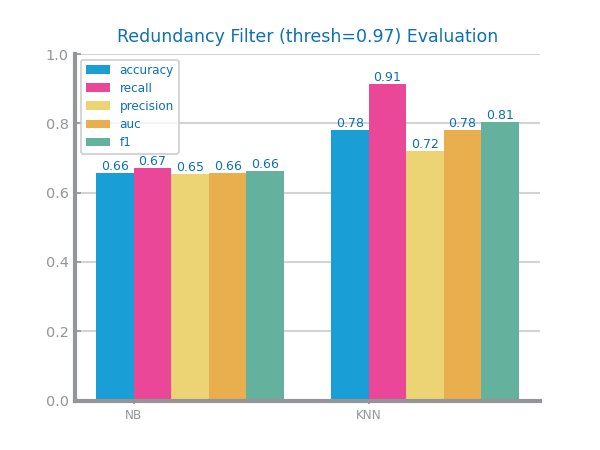
\includegraphics[width=\textwidth]{../images/lab3/flights/6_selection_redundancy_eval.png}
    \caption{Redundancy Analysis}
\end{subfigure}
\caption{Detailed feature selection evaluation - Flights}
\end{figure}

\begin{figure}[H]
\centering
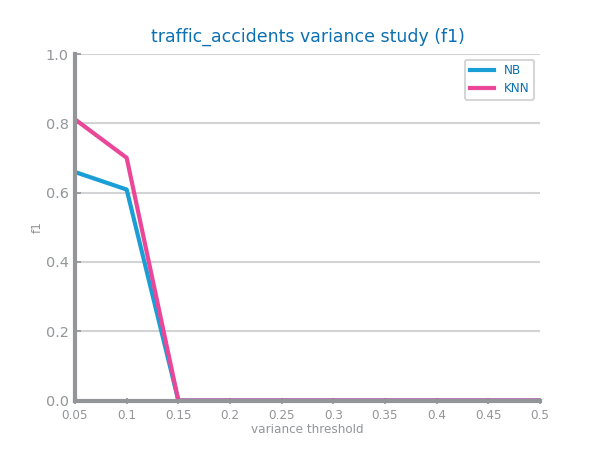
\includegraphics[width=0.85\textwidth]{../images/lab3/flights/6_selection_variance_f1.png}
\caption{Variance study for feature selection - Flights}
\end{figure}

\begin{figure}[H]
\centering
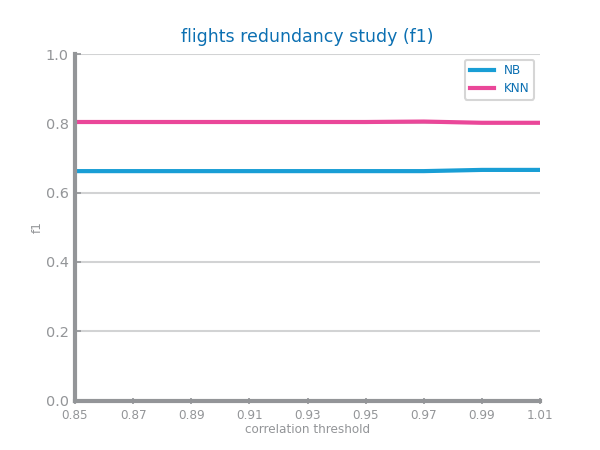
\includegraphics[width=0.85\textwidth]{../images/lab3/flights/6_selection_redundancy_f1.png}
\caption{Redundancy study for feature selection - Flights}
\end{figure}

\begin{figure}[H]
\centering
\begin{subfigure}{0.48\textwidth}
    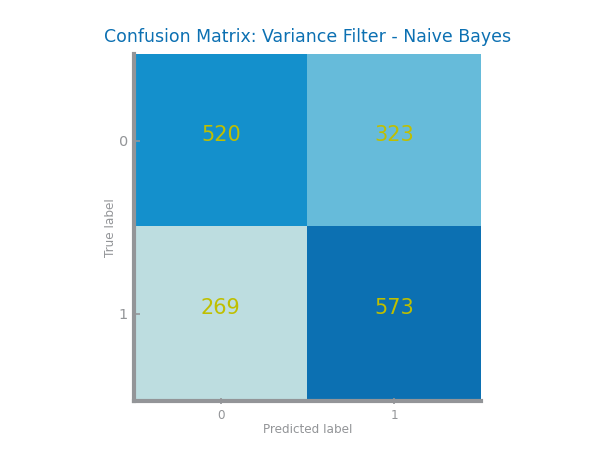
\includegraphics[width=\textwidth]{../images/lab3/flights/6_selection_best_nb_cm.png}
    \caption{Naive Bayes Confusion Matrix}
\end{subfigure}
\hfill
\begin{subfigure}{0.48\textwidth}
    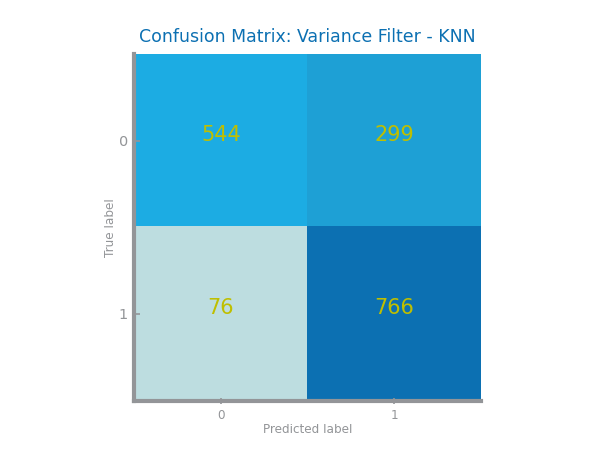
\includegraphics[width=\textwidth]{../images/lab3/flights/6_selection_best_knn_cm.png}
    \caption{KNN Confusion Matrix}
\end{subfigure}
\caption{Confusion matrices for best feature selection - Flights}
\end{figure}

\end{document}